\chapter{Literature Review}
\label{lit_review} % For referencing the chapter elsewhere, use \ref{intro} 
This chapter provides a review of all related works in the field of recommender systems. The chapter first focuses on the background and origin of recommender systems and outlines their main applications. This is then followed by an overview of the methods used to evaluated the accuracy and effectiveness of recommender systems. Then, the two main categories of approaches to recommender systems are discussed, namely \textit{content-based} and \textit{collaborative filtering} systems. Finally, the chapter is concluded by evaluating the top submissions to the Netflix Prize, a contest that held in 2008, which was a major event in the progression of collaborative filtering algorithms.

\section{Introduction to Recommender Systems}
As the world has become more digitally connected, people too have become connected to an increasing number of options. When trying to decide on what movie to watch, or what album to listen to, people are presented with a vast number of options that can, oftentimes, be overwhelming. To help people in making decisions such as these, inspiration is often taken from friends' word of mouth, reviews from critics, or general surveys. Recommender systems provide an automated means for helping people discover new items. \parencite{rs_1.1_Resnick}

The goal of a recommender system can be defined as predicting the response of a user for new items, based on historical information, and suggesting novel and/or original items for which the estimated response is positive \parencite{handbook_1.4_neighbourhood}.

\subsection*{Approaches to Recommender Systems}
Recommender systems can be divided into two broad categories. \textbf{Content based} recommender systems make use of meta data for generating recommendations. Examples of item meta data include the genre of a musical artist or song, or the director of a movie. For users, meta data such as demographic information might be used. This meta data is used to match users to items based on matching tags - a user who likes the work of a certain author will be recommended other books by that same author, or books in the same genre as what they already like. \parencite{di2012linked}

There have been a number of successful content based recommender systems. Many web recommenders use a keyword-based technique, to match web pages based on the frequency of words on the page. In movie and book recommenders, a common approach is to use similarities between the text descriptions to match products. \parencite{handbook_1.3_content-based}

One major obstacle to content based approaches is the lack of sufficient meta data, which can be time-consuming and costly to collect. \parencite{cf_1.6_implicit}

An alternative approach, known as \textbf{collaborative filtering} (CF), uses only the historical interaction behaviour between users and items to make recommendations \parencite{cf_1.1}. This is the approach that will be investigated in this project.

\section{Evaluating Recommender Systems}
Before expanding on the intricacies of collaborative filtering, it is first necessary to discuss the methods and metrics that are commonly used to evaluate recommender systems. This is the most subjective aspect of the process, since the success of the system depends on the objectives of its designer. For example, the intent could be to stretch customer spend, or it could be to encourage users to discover new products. In each of these cases, success would be measured using different yard sticks. \parencite{eval_colab}

There are three main approaches for evaluating the success of a recommender system. The first approach is to evaluate the system offline, without any form of user testing. The other two approaches involve user testing; either using small groups of subject matter experts, or a more large-scale scale approach using online user testing. While each recommender system can be evaluated subjectively based on its ability to meet certain outcomes, there are certain measurable properties which can be used to compare different systems. \parencite{handbook_1.8_evaluation} The intended outcomes of the recommender system will determine whether it can be evaluated offline, or if it will require expert or user group online testing.

\subsection{Offline Evaluation}
Most recommender systems are scored and assessed on their ability to predict user ratings. In this case, the models have been trained to predict the numeric values of ratings that users will assign to items. The predicted values can be compared to the true ratings using common regression metrics such as mean absolute error (MAE) or root mean square error (RMSE). \parencite{eval_coverage} If we use $P$ and $O$ to denote the ordered sets of predicted and observed user rating respectively, and $n$ to represent the total number of user-item interactions, then the accuracy of the recommender system can be calculated as follows:

\begin{equation}
    MAE = \dfrac{|P - O|}{n}
\end{equation}

\begin{equation}
    RMSE = \sqrt{\dfrac{(P - O)^{2}}{n}}
\end{equation}

However, there are alternative metrics which have been formulated that aim to better reflect the quality perceived by users of the system \parencite{eval_colab}.

Prediction \textbf{coverage} provides a measure of how well the recommender system is able to encourage users to explore all of the item space. If $I$ is used to denote all items available to users and $I_p$ to denote all items recommended by the recommender system, then coverage can be calculated as follows:

\begin{equation} \label{eqn:cov}
    coverage = \dfrac{|I_p|}{|I|}
\end{equation}
\hspace{2em} which is the total number of items recommended by the system divided by the total number of items contained in the training data \parencite{eval_coverage}.

In some cases, a recommender system could achieve high levels of both accuracy and coverage, but still struggle to recommend new items to users. \cite{eval_colab} used the example of a recommender system that suggests bananas to shoppers in a grocery store: \textit{"Statistically, this recommendation is highly accurate: almost everyone buys bananas. However, everyone who comes to a grocery store to shop has bought bananas in the past, and knows whether or not they want to purchase more. Further, grocery store managers already know that bananas are popular, and have already organised their store so people cannot avoid going past the bananas."} 

It should be noted, however, that a recommender system should not \textit{only} recommend unexpected items. As \cite{swearingen2001beyondalgorithms} showed, non-novel recommendations help to develop trust from users in the system and should be combined with more unexpected suggestions to provide an enjoyable overall user experience.

\textbf{Serendipity} is a metric that has been used to assess both a recommendation's unexpectedness \textbgf{and} its usefulness \parencite{online_predicting}.

Serendipity is more of a conceptual evaluative measure, rather than a fixed formula like RMSE. One suggested approach to capture serendipity numerically has been suggested by \parencite{eval_colab}. In the case where a recommender can produce expected probabilities for a given user for every item in the system, one could divide each probability by the average user probability score to produce re-weighted scores. The resulting probabilities would represent a measure of how much more likely a given user is to like items than the average user.

In the case where ratings are not available - that is when only a list of user-item interactions is given - the task of providing recommendations is often transformed into one of providing a set number of items to a user. Using the $P$ to denote the items that are suggested to the user and $O$ to denote items which the user was observed to have preferred, this type of approach can then be evaluated using \textbf{precision} and \textbf{recall} as follows: \parencite{handbook_1.4_neighbourhood}

\begin{equation}
    precision = \dfrac{(P + O)}{P}
\end{equation}

\begin{equation}
    recall = \dfrac{(P + O)}{O}
\end{equation}

\subsection{Online Testing}
Testing recommender systems in an online manner, be it user studies or large-scale trials, requires a large enough audience that can be split into test and control groups. Ideally, the two user groups would be identical apart from the fact that the test group would receive suggestions from the recommender system, while the control group would not. The two groups would then be assessed on their behaviour over a trial period, allowing for the recommender system to be assessed in various areas such as uplift in incremental sales or exploration of the item space. \parencite{online_predicting}

An example of online testing can be found in the work done by \cite{swearingen2001beyondalgorithms}, where users were asked to evaluate a number of internet recommender systems and compare their suggestions to those of their friends'. Users were asked to classify which recommendations they received were good, and then to further distinguish between \textbf{useful} recommendations they had never seen before and \textbf{previously liked} recommendations. One particularly interesting observation from this study was that recommender systems tended to produce more suggestions of completely new items than friends, who tended to recommend items of which users were already aware.

The advantage of testing recommender systems in this way is that it affords the systems the chance to influence users' interaction behaviour, which is essentially the ultimate goal. Recommender systems exist for the main purpose of suggesting items to users that they are predicted to like, but would otherwise not have known about. The influence of a recommender system cannot be assessed through back-testing, it can only be done through online trials. \parencite{handbook_1.4_neighbourhood}

Since each system needs its own independent test group, the size of the audience required only increases with the number of recommender systems being compared, which makes online testing unfeasible in the context of this master's dissertation. Therefore, all comparisons between recommender systems in this paper will be made using offline metrics.

\subsection{Netflix Prize}
A major event in the progression of recommender system methods, as well as the evaluative metrics thereof, was the 2006 Netflix Prize. In 2019, Netflix is a well-known online video subscription service that provides content to subscribers through streaming. However, in 2006 Netflix was an online video subscription service that provided DVD rentals to subscribers via the mail. As part of their service, they encouraged users to rate movies that they watched which resulted in the creation of a data set of some 1.9 billion ratings from 11.7 million subscribers across 85 thousand titles in under 10 years. \parencite{netflix_description}

This data set was used by Netflix to create their own recommendation algorithm, which was known as Cinematch. Cinematch used a variant of Pearson's correlation to determine a movie's similarity to all other movies. These similarities between movies were used to provide personalised recommendations to users based on the movies they had rated. The main method used to assess the performance of Cinematch was to compute the RMSE between the predicted and observed user ratings. \parencite{netflix_description}

Then, in 2006, Netflix released a variation of this data set to the data science community at large with the challenge of improving on the performance achieved by the existing Cinematch algorithm. The data set provided for this challenge contained over 100 million ratings (and their dates) from over 480 thousand subscribers on almost 18 thousand movies. The data were collected between 1998 and 2005 comprised a representative sample of all ratings captured by Netflix during this period. The user ratings were measured on an integer scale from 1 to 5. 3 million of the most recent ratings from those same subscribers across the same set of movies was withheld as a competition qualifying set. Half of the qualifying data set was used to compute the RMSE of submissions onto the running public leader board, while the other half, known as the "quiz" subset was used by Netflix to decide the eventual winning team. \parencite{netflix_description}

As a reference for competition contestants, Netflix reported that the Cinematch algorithm was able to achieve a performance of 0.9514 RMSE on the quiz subset, which was 9.6\% lower than simply predicting using the average movie ratings. \parencite{netflix_description}

\begin{figure}[H]
\centering
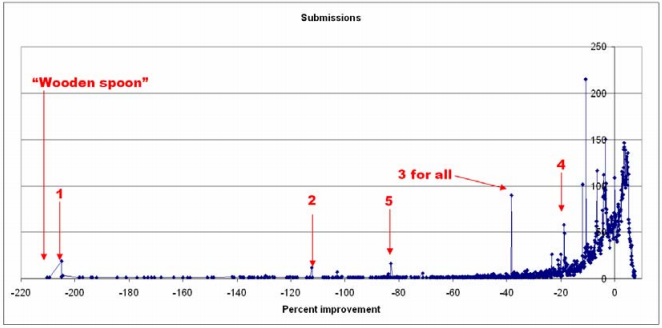
\includegraphics[width=13cm]{Figures/2_1_netflix-prize.png}
\decoRule
\caption[Netflix submissions]{Netflix prize submissions ordered by improvement over Cinematch \parencite{netflix_description}.}
\label{fig:netflix_submissions}
\end{figure}

Figure \ref{fig:netflix_submissions} above shows the relative distribution of the submissions' performance with respect to that of the Cinematch algorithm. The figure above was created in 2007, at which point no team had achieved the goal of a 10\% improvement over Cinematch. The numbers in red correspond to submissions in which the same value is used for every prediction. Interestingly, a significant number of submissions achieved RMSE scores lower than would be achieved by predicting every rating to be 4.

However, in 2008, the competition reached its conclusion, when the team known as "BellKor's Pragmatic Chaos" surpassed the 10\% improvement level \parencite{netflix_bellkor}.

\section{Collaborative Filtering}
The term 'collaborative filtering' was first coined in 1992, when D. Goldberg \textit{et al.} used it to refer to a system for suggesting relevant emails for a person from a selection of mailing lists. This system incorporated the reactions of other users in the filtering process. \parencite{cf_1.3_origin}

Since then, the term has generally been used to describe a process through which known preferences of users in a group are used to predict the unknown preferences of other users \parencite{cf_1.1}. In most cases, the preferences of users within the group are indicated by a rating or score of some kind; users will assign positive ratings to items they liked, and negative ratings to items they did not. The term \textit{collaborative} refers to the fact that the users of the system improve its performance with each rating that they contribute \parencite{cf_1.2_eigentaste}, i.e., as users record more ratings of items, the ability of the system to \textit{filter} accurate recommendations for other users improves. 

Collaborative filtering techniques provide an algorithmic method for making recommendations to users, based on the preferences of other similar users. The fundamental assumption that underlies CF techniques is that users who have both rated $k$ items similarly will also rate other items similarly too. For example, if user $A$ likes movies $m_1$, $m_2$, $m_3$, and user $B$ likes movies $m_1$, $m_2$, $m_3$, $m_4$, then user $A$ is also likely to enjoy movie $m_4$.

One of the advantages of collaborative filtering is that it can be performed without any meta data relating to either the users or the items in the database. Whereas other predictive models make predictions for a response variable using the values of one or more predictor variables, CF models make predictions for ratings, using only other ratings.

\subsection{User Feedback}
 In collaborative filtering recommender systems, the inputs are provided by people (users) who rate items with which they have interacted. The function of a recommender system is to aggregate these ratings from users to make recommendations to other users on which items they might like. In some cases, ratings are provided to a recommender system explicitly by users, but in many other cases these ratings have to be inferred based on user-item interactions. 

\subsubsection{Explicit Ratings}
Explicit feedback is captured when a user makes the conscious decision to \textit{explicitly} rate an item. These ratings can be binary, e.g. like or dislike, numeric, e.g. 1-10 rating scale, or unstructured, e.g. annotated text. For example, a user can indicate that they like a certain song by giving it a "thumbs up" on a music streaming service.

This type of feedback directly captures user preferences towards items; however, it can be scarce. It has also been found that the rate at which users provide explicit feedback decreases over time and, furthermore, that leaving feedback has a negative effect on user behaviour overall \parencite{cf_1.5_explicit}.

\subsubsection{Implicit Feedback}
Alternatively, the user might not explicitly rate items they like, in which case a recommender system would need to infer their preferences from their interaction history. Using the example of a music streaming service, many users do not choose to 'like' or rate songs; however, they will tend to listen to songs they like more often than those they do not. \cite{cf_1.5_explicit}, showed that there is a positive correlation between the number of 'likes' a track receives from users and its total play count. Therefore, it is a viable option to infer positive feedback from user interaction data. Other forms of implicit feedback include purchase history, browsing and search patterns, or mouse movements and click patterns \parencite{handbook_1.5_cf}.

Whether the user feedback is implicit or explicit, the job of the recommender system is the same - to aggregate this feedback from users to aid others in discovering new items of interest. It has been shown that using a combination of explicit and implicit feedback can yield improved recommendation accuracy \parencite{cf_1.4_comparison}; however, it is the subtleties around \textit{how} recommender systems identify all the signals from the available user feedback data that remains the greatest area of focus for improving accuracies.

\subsection{Neighbourhood-based Recommender Models}
There are two main techniques used in collaborative filtering recommender systems: \textit{neighbourhood-based} and \textit{latent factor} models \parencite{handbook_1.5_cf}. As the name suggests, neighbourhood models employ a nearest-neighbours approach to recommending items to users.

One issue with content-based approaches is their limited capacity to recommend novel, unexpected items. The system will recommend items which match highly to a user's known preferences, i.e. they are limited by the user's tendency for exploration. \parencite{handbook_1.3_content-based}

Neighbourhood-based models, on the other hand, leverage the collective experiences of all users to recommend interesting new items to users. The principle idea is that two users will rate a particular item similarly if they have rated other items similarly too. Therefore, the weakness of content-based models is the strength of collaborative filtering models, since the user group will inevitably cover more of the item space as a whole than each person individually.



\subsubsection{User-based similarity}
\subsubsection{Item-based similarity}

\subsection{Latent Factor Recommender Models}

\subsection{Commonly Used Data Sets for Recommender Systems}